\chapter{安装并搭建环境}

\section{简介}
Python是通用、解释型高级计算机程序设计语言,融合结构化、面向对象、及函数式编程特征,主要特征是面向对象。该语言由荷兰人Guido van Rossum(BDFL, Benevolent Dictator For Life)创制,1991年发行第一个公开版本。之后,持续发展,衍生出2.x和3.x两个系列。

\section{python版本}
\begin{itemize}
\item python版本有两个系列,2.x与3.x,互不兼容
\item \href{https://pythonclock.org/}{python倒计时}
\item 学习、使用3.x
\end{itemize}

\section{安装}
\subsection{Windows}
Anaconda Suite for Windows,下载地址: \url{https://www.anaconda.com}
\subsection{Linux}
\begin{itemize}
\item Linux发行版自带Python2.x,使用Python3.x需另安装
\item 若安装Anaconda Suite for Linux,不用操心版本、扩展库兼容问题
\item 安装指南:\href{https://poweruphosting.com/blog/install-anaconda-python-ubuntu-16-04/}{How to Install anaconda in ubuntu 16.04}
\end{itemize}
\subsection{虚拟环境}
\begin{description}
\item{pyvenv:} A tool to create isolated virtual environments from a Python interpreter. Ships with Python from 3.4.
\url{https://docs.python.org/3/library/venv.html}
\item{virtualenv:} Creates virtual environments, available in PyPi. It can installs different versions of Python interpreters \url{https://pypi.python.org/pypi/virtualenv}
\end{description}

\section{编程环境}
\begin{itemize}
\item Jupyter Notebook
\item IDLE
\item command line
\item github: 参考\footnote{\protect\href{https://github.com/geeeeeeeeek/git-recipes}{高质量的Git中文教程}} 
\item 记笔记: EverNote,WizNote,博客,各种云盘
\item 展示代码运行工具: \url{www.pythontutor.com}
\end{itemize}

\section{练习}
\subsection{交互模式}
\begin{python}
  print('Hello, World!')

  # print python version
  import sys
  sys.version
  # sys.winver for Jupter Notebook only
  sys.version_info
\end{python}
\subsection{脚本模式}
\inputpython{examples/hello.py}{5}{7}

\section{编程话题}
\subsection{编程要掌握哪些技能}
\begin{itemize}
\item 计算思维\footnote{Allen Downey, Jeffrey Elkner, Chris
    Meyers. \protect\href{http://openbookproject.net/thinkcs/python/english3e/index.html}{How
      to Think Like a Computer Scientist}, Oct,2002}Computational
  thinking.
\item 阅读并理解别人的代码 Understand code.  Reading code is one of the
  best way to learn programming, beside writing code.
\item 理解计算的能与不能 Understand limits and abilities.  Something(not
  everything) can be computed. % 例如,浮点数
\item 解决问题 Map problem into computational solution. 
  \begin{compactenum}
    \item 观察、提出问题
    \item 分析问题、提出方案
    \item 设计实验、实施方案
    \item 分析结果及反馈
  \end{compactenum}
\end{itemize}
\subsection{知识的类别}
\begin{description}
\item{陈述式知识:} 有关事实和情况的说明。
  \begin{compactenum}
  \item 例: 饭店的菜肴介绍,包括配料成分、色香味、照片
  \item 例: 算术,包括数字:自然数、有理数等;及算符:加减乘除等
  \end{compactenum}
\item{程序式知识:} 有关完成某件工作的一系列操作步骤的描述,这些描述用一系列步骤刻画\emph{计算过程}。
  \begin{compactenum}
  \item 例: 菜肴的烹制方法和过程,各种相关操作及其执行顺序,西红柿炒蛋
  \item 例: 四则运算法则,先乘除后加减
  \end{compactenum}
\item {计算机做的计算:} 就是刻画程序式知识的方法。
  \begin{compactenum}
  \item 欧几里德算法又称辗转相除法,用于计算两个整数m, n的最大公约数。其计算原理依定理:gcd(m, n) = gcd(n, m mod n)。这个定理的意思是:整数m、n的最大公约数等于n和m除以n的余数的最大公约数。
  \item 例: 有两个整数:120和45,我们按照上面的方法求他们的最大公约数。 \\
    1. gcd(120, 45) = gcd(45, 120 mod 45) = gcd(45, 30) \\
    2. gcd(45, 30) = gcd(30, 45 mod 30) = gcd(30, 15) \\
    3. gcd(30, 15) = gcd(15, 30 mod 15) = gcd(15, 0) = 15 \\
    当 m mod n 等于零时,即求15和0的最大公约数时,这个循环应该终止,15就是120和45的最大公约数。
    算法强调\emph{计算过程},而非计算结果。
  \end{compactenum}
\item {编程:} 将过程式知识,通过计算机程序设计语言表示出来,存储在文件中,并且可执行。
\end{description}
\subsection{怎么编程序?}
编程: 告诉计算机做什么。程序用某种计算机能理解的语言编写算法,输入计算机,计算机编译或解释执行语言,实现功能。

算法: 类似菜谱、说明手册,详细说明做事步骤。

例如: 西红柿炒蛋
\begin{verbatim}
  放入鸡蛋翻炒
  放入西红柿
 如果 没熟:
    继续翻炒
    直至熟了,不再翻炒
  加盐调味
  如果 不入味:
    继续加盐
    直至口感合适
  出锅盛盘
\end{verbatim}
该算法包含原料,如鸡蛋、西红柿、盐,代表被操作的数据,及程序指令,如放入、翻炒、加盐、出锅,代表操作动作。

例如:\Cref{Euclideanalgorithm}欧几里得法
\begin{figure}
  \centering
  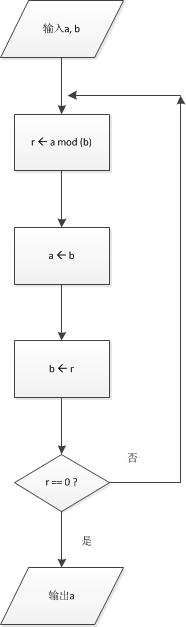
\includegraphics{diagrams/EuclideanAlgorithm.jpeg}
  \caption{欧几里得算法流程图}
  \label{Euclideanalgorithm}
\end{figure}
版权允许情况下,算法、程序可自由修改、发布、分享。在自由软件(Free software)、开源(Open source)、社会化编程(Social programming)影响下,获得、学习、改进开源程序成为风尚。
\subsection{计算机程序设计语言}
1936年,Alan Turing认为用6条基本指令,一切都可以解决。由此推论,只要能在一种语言中实现,就能在另一种语言中实现。 C中能实现的没有Fortran不能实现的。这称为“图灵兼容”(Turing compatible)。 这个论断表明语言只是工具,图灵兼容意义上无差别,只不过,实际使用,每种语言有其特别适用处。

语言分类: 高级语言 vs. 低级语言;通用 vs. 专用;编译型 vs. 解释型; 过程式 vs. 面向对象 vs. 函数式。

\section{课后阅读}
\begin{itemize}
\item 访问\href{https://www.python.org}{Python官网}
\item 阅读\href{https://wiki.python.org/moin/BeginnersGuide}{《新手指南》}
\item 阅读\href{https://docs.python.org/3/tutorial/}{《入门指南》}
\item 访问\href{http://www.anaconda.com}{Anaconda官网}
\item 了解\href{https://docs.anaconda.com/}{Anaconda文档}
\item 阅读《计算机科学导论》
\end{itemize}
